%%%%%%%%%%%%%%%%%%%%%%%%%%%%%%%%%%%%%%%%%
% Friggeri Resume/CV
% XeLaTeX Template
% Version 1.2 (3/5/15)
%
% This template has been downloaded from:
% http://www.LaTeXTemplates.com
%
% Original author:
% Adrien Friggeri (adrien@friggeri.net)
% https://github.com/afriggeri/CV
%
% License:
% CC BY-NC-SA 3.0 (http://creativecommons.org/licenses/by-nc-sa/3.0/)
%
% Important notes:
% This template needs to be compiled with XeLaTeX and the bibliography, if used,
% needs to be compiled with biber rather than bibtex.
%
%%%%%%%%%%%%%%%%%%%%%%%%%%%%%%%%%%%%%%%%%

\documentclass[]{friggeri-cv} % Add 'print' as an option into the square bracket to remove colors from this template for printing

\addbibresource{gkiarcv.bib} % Specify the bibliography file to include publications

\begin{document}

\header{gregory}{kiar}{biomedical engineer} % Your name and current job title/field

%----------------------------------------------------------------------------------------
%	SIDEBAR SECTION
%----------------------------------------------------------------------------------------

\begin{aside} % In the aside, each new line forces a line break
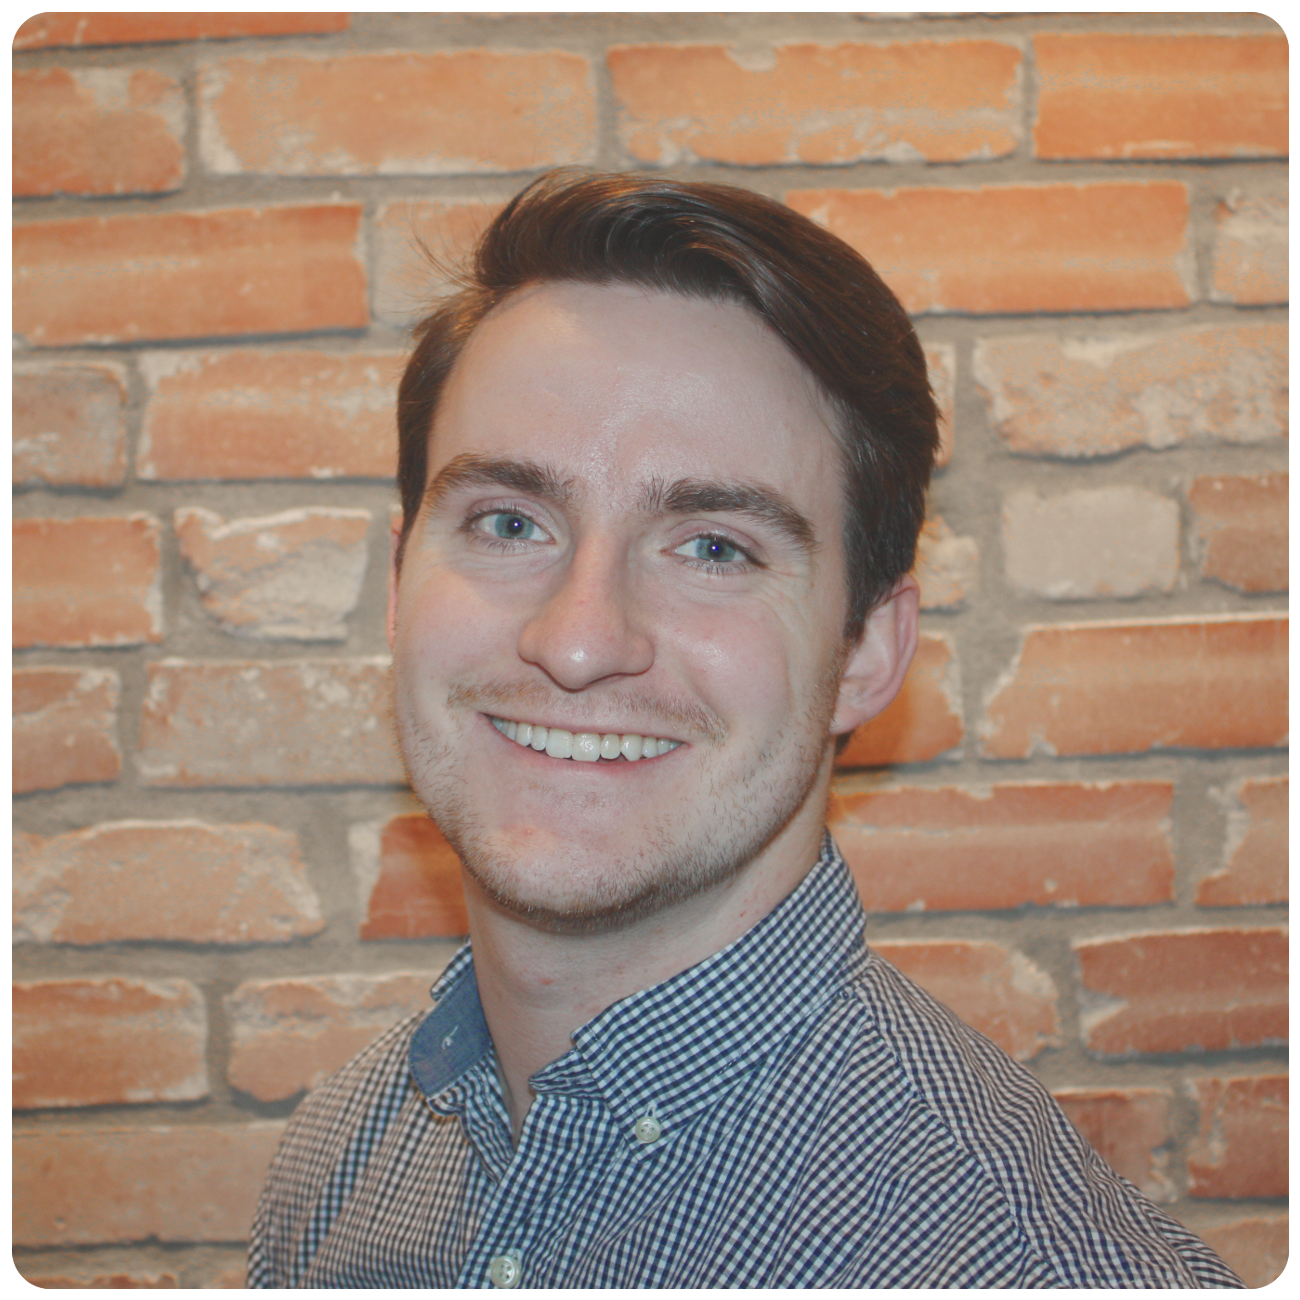
\includegraphics[width=\textwidth]{./headshot_shorthair.png}
\section{contact}
3801 University Street
NW 144/145
Montreal, Quebec
H3A 2B4, Canada
~
\href{mailto:gkiar07@gmail.com}{greg.kiar@mcgill.ca~{\color{red} \faEnvelope}}
\href{http://gkiar.github.io}{gkiar.me~{\color{lightblue} \faGlobe}}
\href{http://github.com/gkiar}{gkiar~{\color{purple} \faGithub}}
\href{https://twitter.com/g_kiar}{{\color{blue} \faTwitter}} \href{https://www.linkedin.com/in/gregkiar}{{\color{green} \faLinkedin}} \href{https://publons.com/author/1305375/gregory-kiar#profile}{{\color{plubblue} \aiPublons}} \href{http://orcid.org/0000-0001-8915-496X}{{\color{orcidgreen} \aiOrcid}} \href{https://scholar.google.com/citations?user=ztw6g7kAAAAJ&hl=en}{{\color{googred} \aiGoogleScholar}} \href{https://www.researchgate.net/profile/Gregory_Kiar}{{\color{gateteal} \aiResearchGate}}
\section{languages}
english native speaker,
basic ASL
\section{programming}
Python, R, Bash {\color{red} $\varheartsuit$}
MATLAB, C++, AWS,
Ruby, LaTeX, etc.
\section{soft skills}
leadership, teaching, sci.~comm., design, problem~solving
\end{aside}

%----------------------------------------------------------------------------------------
%	EDUCATION SECTION
%----------------------------------------------------------------------------------------

\section{education}

\begin{entrylist}

%------------------------------------------------

\entry
{2017 -- now}
{PhD candidate {\normalfont in Biomedical Engineering}}
{McGill University, Montreal, QC}
{Thesis work supervised by Alan Evans and Tristan Glatard on a project entitled:\\ Characterizing the Stability of
Neuroimaging Analyses Through Perturbations in Experimental Design.
All code and data have been made publicly available.}

%------------------------------------------------

\entry
{2014 -- 2016}
{M.S.E {\normalfont in Biomedical Engineering}}
{Johns Hopkins University, Baltimore, MD}
{Thesis work was supervised by Joshua T. Vogelstein on a project entitled:\\GREMLIN:
Graph Estimation from MR images Leading to Inference in Neuroscience. All code and data have
been made publicly available.}

%------------------------------------------------

\entry
{2010 -- 2014}
{B.Eng {\normalfont in Biomedical and Electrical Engineering}}
{Carleton University, Ottawa, ON}
{Capstone work was supervised by Leonard MacEachern on a project entitled:\\Electrical
muscle stimulation with concurrent EMG feedback of the upper arm for applications in stroke
rehabilitation.}

%------------------------------------------------

\entry
{2018}
{Software and Data Carpentry Instructor Training}
{Compute Canada, Toronto, ON}
{Running workshops in the context of an evidence-based instructional pedagogy.}

%------------------------------------------------

\entry
{2016}
{Exploring the Human Connectome}
{The Human Connectome Project, Boston, MA}
{Development and deployment of connectome estimation pipelines.}

%------------------------------------------------

\entry
{2015}
{Presenting Data and Information}
{Edward Tufte, Baltimore, MD}
{Cultivate skills in effective communication with scientific figures.}

\end{entrylist}

%----------------------------------------------------------------------------------------
%	WORK EXPERIENCE SECTION
%----------------------------------------------------------------------------------------

\section{experience}

\subsection{Academic Experience}

\subsubsection{}{Current Positions \& Activities}

\begin{entrylist}
\entry
{05/17 -- now}
{McGill Centre for Integrative Neuroscience (MCIN)}
{Montreal, QC}
{\job{Software Developer \& Researcher} \\
Responsible for the exploration and integration of distributed software software services with high
performance computing clouds and clusters, providing development, training, and support towards the
use of tools and services within international collaborations, and developing methods for evaluating
and describing analysis software in neuroimaging.}
 % \end{entrylist}

 %\subsubsection{}{Current Activities}

 %\begin{entrylist}
\entry
{06/18 -- now}
{Organization for Human Brian Mapping (OHBM)}
{Minneapolis, MN}
{\job{Treasurer - Open Science Special Interest Group} \\
Responsible for the procurement and management of finances for the special interest group. Includes
creating budgets, interfacing with sponsors and vendors, as well as event organizers for the various
activities run by the Open Science special interest group.}
\end{entrylist}

\newgeometry{left=2cm, bottom=2.5cm, right=1.5cm}
\renewcommand{\bfseries}{\headingfont\color{headercolor}}
\renewcommand{\entry}[4]{%
  #1&\parbox[t]{15.7cm}{%
    \textbf{#2}%
    \hfill%
    {\footnotesize\addfontfeature{Color=lightgray} #3}\\%
    #4\vspace{\parsep}%
  }\\}

% add this below the last entry on your first page
% \newgeometry{left=2cm, bottom=2.5cm, right=1.5cm}
\renewcommand{\bfseries}{\headingfont\color{headercolor}}
\renewcommand{\entry}[4]{%
  #1&\parbox[t]{15.7cm}{%
    \textbf{#2}%
    \hfill%
    {\footnotesize\addfontfeature{Color=lightgray} #3}\\%
    #4\vspace{\parsep}%
  }\\}

% add this below the last entry on your first page
% \newgeometry{left=2cm, bottom=2.5cm, right=1.5cm}
\renewcommand{\bfseries}{\headingfont\color{headercolor}}
\renewcommand{\entry}[4]{%
  #1&\parbox[t]{15.7cm}{%
    \textbf{#2}%
    \hfill%
    {\footnotesize\addfontfeature{Color=lightgray} #3}\\%
    #4\vspace{\parsep}%
  }\\}

% add this below the last entry on your first page
% \input{midamble.tex}



\clearpage
\subsubsection{}{Previous Positions}

\begin{entrylist}
\entry
{09/14 -- 05/17}
{Center for Imaging Science, Johns Hopkins University}
{Baltimore, MD}
{\job{Research Engineer}\\
Development and maintenance of an open-source pipeline for structural connectome estimation in humans
and implemented statistical algorithms for quality control of data derivatives. Publicly released data
products to lower the barrier to entry for neuroscience research. Chiefly responsible for grant reporting
and public presence at conferences and workshops.}

\entry
{06/13 -- 09/13}
{Dept. of Systems and Computer Engineering, Carleton University}
{Ottawa, ON}
{\job{Research Assistant with Dr. Rafik Goubran}\\
Developed wireless medical data publish-subscribe system for viewing patient vital signs remotely.}

\entry
{06/12 -- 09/12}
{Dept. of Systems and Computer Engineering, Carleton University}
{Ottawa, ON}
{\job{Research Assistant with Dr. Andy Adler}\\
Utilized neural networks for inverse modeling of real and simulated biological systems.}

\entry
{06/11 -- 09/11}
{Dept. of Biology, Carleton University}
{Ottawa, ON}
{\job{Research Assistant with Dr. Jeffrey Dawson}\\
Developed robotics platform for studying insect locomotion patterns and behaviour.}

\entry
{01/09 -- 09/09}
{CRC, Ottawa Hospital Research Institute}
{Ottawa, ON}
{\job{Research Assistant with Dr. Jim Dimitroulakos}\\
Tested combination therapies of Lovastatin and Cisplatin drugs on colon and breast cancer strains.}
\end{entrylist}

\subsection{Teaching Experience}

\begin{entrylist}
\entry
{05/17 -- now}
{McGill University, OHBM, Brain Intensive, others}
{Montreal, QC}
{\job{Neuroinformatics Instructor} \\
Regularly plan and teach a series of workshop introducing neuroscientists and trainees to methods in neuroinformatics.
Developed and publicly released all course content on GitHub under the "Brainhack101" moniker and several videos on
YouTube under the "BrainIntensive" profile.}

\entry
{09/14 -- 05/17}
{Dept. of Biomedical Engineering, Johns Hopkins University}
{Baltimore, MD}
{\job{Teaching Assistant} \\
Responsible for instruction, evaluation, and content design for: Freshman Modeling and Design
for BME (2014, 2015), Systems and Controls (2015), Statistical Connectomics (2015), The Art of
Data Science (2016), NeuroData Design (2016). Spent more than 500 hours working with students.}

\entry
{01/\{15, 16, 17\}}
{Dept. of Computer Science, Johns Hopkins University}
{Baltimore, MD}
{\job{Instructor}\\
Responsible for instruction, evaluation, and content design for intensive 3-week project-based course on an
introduction to connectomics research across multiple scales and experimental modalities. Spent more than 300 hours
planning, designing course content, and working with students.}

\entry
{09/12 -- 05/14}
{Student Academic Success Center, Carleton University}
{Ottawa, ON}
{\job{Facilitator for Peer-Assisted Study Sessions}\\
Instructed and demonstrated mastery of principles in electromagnetism and power engineering. Spent more than 300 hours
working with students.}

\entry
{08/13 -- 05/14}
{Student Academic Success Center, Carleton University}
{Ottawa, ON}
{\job{Facilitator Team Leader}\\
Provided training, mentoring, and coaching to student instructors in a variety of disciplines. Spent more than 100
hours training and working with facilitators.}
\end{entrylist}

\begin{entrylist}
\entry
{01/13 -- 06/14}
{Dept. of Systems and Computer Engineering, Carleton University}
{Ottawa, ON}
{\job{Teaching Assistant}\\
Instructed introductory level C++ programming. Led lab sessions and instructional workshops. Spent more than 300 hours
working with students.}
\end{entrylist}


%----------------------------------------------------------------------------------------
%	EXTRACURRICULARS SECTION
%----------------------------------------------------------------------------------------
\section{memberships \& extracurriculars}

\begin{entrylist}
\entry
{2017 -- now}
{OHBM Open Science SIG}
{Minneapolis, MN}
{Treasurer}

\entry
{2017 -- now}
{Canadian Open Neuroscience Platform Training Committee}
{Montreal, QC}
{Trainee Representative}

\entry
{2017 -- now}
{Various Neuroinformatics-based Hackathons and Courses}
{Montreal, QC}
{Hackathon Chair, Organizer, \& Instructor}

\entry
{2017 -- 2018}
{OHBM Open Science SIG}
{Minneapolis, MN}
{Hackathon Chair}

\entry
{2017 -- 2018}
{Healthy Brains for Healthy Lives Trainee Committee}
{Montreal, QC}
{President (Neuroinformatics)}

\entry
{2014 -- 2017}
{NeuroData}
{Baltimore, MD}
{Chief Neurocartographer}

\entry
{2015 -- 2017}
{College Prep Program}
{Baltimore, MD}
{College Mentor, SAT Coach, \& Essay Reviewer}

\entry
{2014 -- 2016}
{Thread}
{Baltimore, MD}
{Grandparent (i.e. supervisor) \& Family Member (i.e. mentor) }

\entry
{2013 -- 2014}
{Carleton University Biomedical Engineering Society}
{Ottawa, ON}
{President}

\entry
{12/12, 12/13}
{Operation Red Nose Ottawa}
{Ottawa, ON}
{Navigator and Driver}

\entry
{2010 -- 2011}
{Carleton University Student Emergency Response Team}
{Ottawa, ON}
{Emergency First Responder}
\end{entrylist}

%----------------------------------------------------------------------------------------
%	AWARDS SECTION
%----------------------------------------------------------------------------------------

\section{awards}

\begin{entrylist}
\vspace{-7pt}

\entry
{2018}
{Michael Smith Foreign Study Supplement}
{NSERC, Ottawa, ON}
{}
\vspace{-7pt}
% $5200
% Rank: 11
% Pillar: Computational Sciences

\entry
{2018}
{Alexander Graham Bell Canada Graduate Scholarship (CGS D)}
{NSERC, Ottawa, ON}
{}
\vspace{-7pt}
% $105000
% Rank: 11
% Pillar: Computational Sciences

\entry
{2017}
{Healthy Brains for Healthy Lives Doctoral Fellowship}
{McGill University, Montreal, QC}
{}
\vspace{-7pt}
% $15000

\entry
{2017}
{CRN Coding Sprint Project Award}
{Stanford University, Palo Alto, CA}
{}
\vspace{-7pt}
% $2000

\entry
{2017}
{OHBM BrainHack Travel Award}
{OHBM, Minneapolis, MN}
{}
\vspace{-7pt}
% $500

\entry
{2014 -- 2016}
{Full-tuition Master's Degree Fellowship}
{Johns Hopkins University, Baltimore, MD}
{}
\vspace{-7pt}
% $100,000

\entry
{2014}
{Graduated with Distinction}
{Carleton University, Ottawa, ON}
{}
\vspace{-7pt}

\entry
{2014}
{Greatest Social Impact Paper}
{Professional Engineering Ontario (PEO), Ottawa, ON}
{}
\vspace{-7pt}
% $500
%{Awarded to the capstone project with the potential to produce the largest positive societal impact.}

\entry
{2014}
{SEED Fund}
{Carleton University Engineering Alumni, Ottawa, ON}
{}
\vspace{-7pt}
% $800
%{Awarded to the capstone project deemed most likely to become a successful startup.}
\end{entrylist}

\begin{entrylist}
\vspace{-7pt}

\entry
{2014}
{IEEE Papers Showcase Local Winner}
{IEEE Ottawa-Carleton Chapter, Ottawa, ON}
{}
\vspace{-7pt}
% $500
%{Awarded to the capstone project best demonstrating mastery of core electrical engineering principles.}

\entry
{2014}
{Carleton Electronics Project Competition Champion}
{Carleton University, Ottawa, ON}
{}
\vspace{-7pt}
%{Awarded to the capstone project best demonstrating mastery of core electrical engineering principles.}

\entry
{2013}
{Engineering '65 and '66 Scholarship}
{Carleton University, Ottawa, ON}
{}
\vspace{-7pt}
% $2,000
%{Awarded to students maintaining a GPA above a 10/12 (the equivalent of an A).}

\entry
{2012 -- 2014}
{Dean's Honour List}
{Carleton University, Ottawa, ON}
{}
\vspace{-7pt}
%{Awarded to students maintaining a GPA above a 10/12 (the equivalent of an A).}

\entry
{2012}
{Clarence C. Gibson Scholarship}
{Carleton University, Ottawa, ON}
{}
\vspace{-7pt}
% $2,000
%{Awarded to students maintaining a GPA above a 10/12 (the equivalent of an A).}
\end{entrylist}


%----------------------------------------------------------------------------------------
%	INTERESTS SECTION
%----------------------------------------------------------------------------------------

\section{interests}

\textbf{professional:} reproducibility, accessibility, high performance computing, neuroscience,
pipeline engineering, big data, data analysis, software design, machine learning, statistics.
\textbf{personal:} guitar, hockey, soccer, design, hiking, paddling.

\section{reviewed for}
\begin{enumerate}
\item Frontiers in Neuroinformatics
\item Gigascience
\end{enumerate}

%----------------------------------------------------------------------------------------
%	PUBLICATIONS SECTION
%----------------------------------------------------------------------------------------
% \clearpage

\section{publications}
\printbibsection{manual}{pre-prints} % Print all articles from the bibliography

\printbibsection{article}{articles in peer-reviewed journals} % Print all articles from the bibliography

\printbibsection{inproceedings}{proceedings in international peer-reviewed conferences} % Print all inproceedings entries from the bibliography

\printbibsection{inbook}{book chapters} % Print all inbook entires

\printbibsection{booklet}{invited talks \& organized workshops} % Print all booklet entries from the bibliography

\printbibsection{proceedings}{posters at international conferences} % Print all proceedings entries from the bibliography

\printbibsection{misc}{published code} % Print all miscellaneous entries from the bibliography

\printbibsection{report}{works in progress} % Print all research reports from the bibliography
%----------------------------------------------------------------------------------------
\end{document}
